\documentclass[12pt]{article}

% Packages
\usepackage{amsmath, amssymb, amsthm}
\usepackage{geometry}
\usepackage{fancyhdr}
\usepackage{enumitem}
\usepackage{titlesec}
\usepackage{caption}
\usepackage{tcolorbox}
\usepackage{float}

% Page Setup
\geometry{margin=1in}
\setlength{\parindent}{0pt}
\setlength{\parskip}{0em}
\setcounter{secnumdepth}{3}

\pagestyle{fancy}
\fancyhf{}
\lhead{Ethan Fan}
\rhead{PCH}
\cfoot{\thepage}

% Section Formatting
\titleformat{\section}
  {\bfseries}
  {}
  {0em}
  {}
\titlespacing*{\section}{0pt}{0pt}{0.3em}

\titleformat{\subsection}[runin]
  {\bfseries}
  {}
  {0em}
  {}
\titlespacing*{\subsection}{0pt}{0pt}{0em}

\titleformat{\subsubsection}[runin]
  {\itshape}
  {(\roman{subsubsection})}
  {0em}
  {}

% mathematical commands
\newcommand{\ddt}{\frac{d}{dt}}
\newcommand{\ddx}{\frac{d}{dx}}
\newcommand{\dydx}{\frac{dy}{dx}}

\newcommand{\definition}[1]{\begin{tcolorbox}[colback=red!5!white,colframe=red!75!black,parbox=false] #1 \end{tcolorbox}}

\newcommand{\theorem}[2]{\begin{tcolorbox}[title={#1},colback=blue!5!white,colframe=blue!75!black,parbox=false] #2 \end{tcolorbox}}

\newcommand{\example}[2]{\begin{tcolorbox}[title={Example: #1},colback=brown!5!white,colframe=brown!75!black,parbox=false] #2 \end{tcolorbox}}

\newcommand{\remark}[2]{\begin{tcolorbox}[title={#1},colback=black!5!white,colframe=black!75!black,parbox=false] #2 \end{tcolorbox}}

% Document
\begin{document}

\vspace*{0cm}

\begin{center}
    {\Large \bfseries Problem Set 54} \\[0.5cm]
    {\large Polar Curves} \\[0.35cm]
    {\normalsize February 17, 2026}
\end{center}

% Questions

\section{Question 2}
Sketch the following curves using the process outlined in problem $\#$1:

\vspace{-1.5em}
\begin{flalign*}
    & \textbf{(a) } r=2(1+\cos \theta) &
\end{flalign*}

\begin{figure}[H]
    \centering
    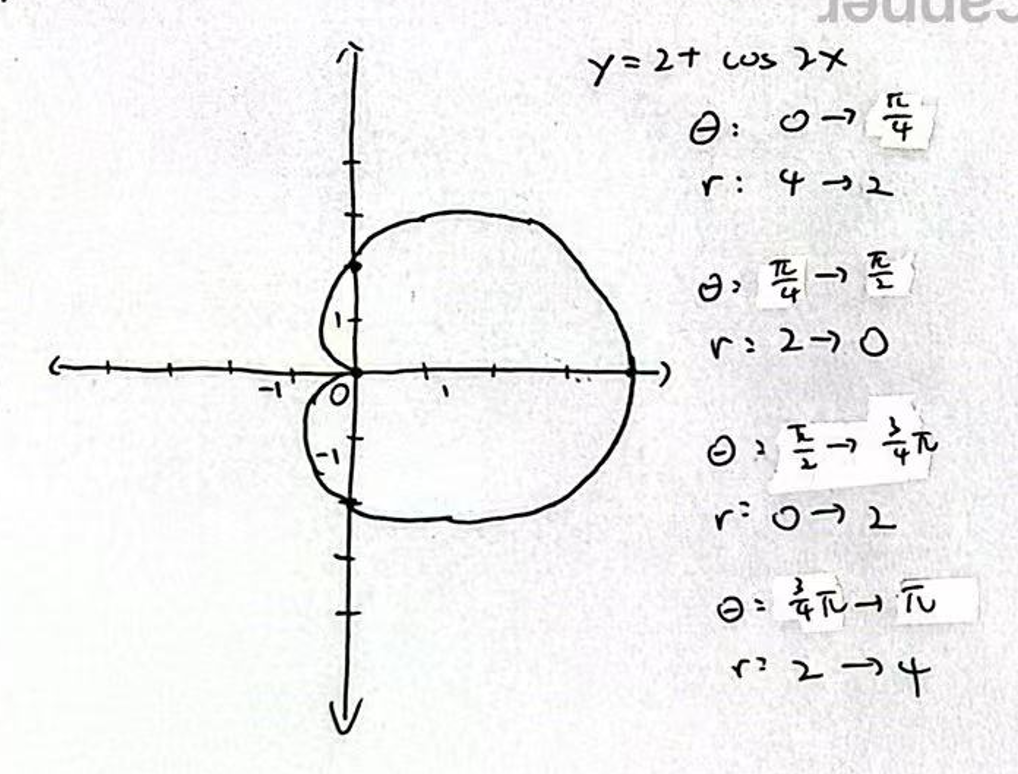
\includegraphics[width=0.5\linewidth]{屏幕截图 2026-02-18 080358.png}
    \caption{2.a}
    \label{fig:placeholder}
\end{figure}

\theorem{Limacon}{
\begin{itemize}
    \item $r=a+b \sin \theta$ or $r=a+b \cos \theta$
    \item Cardioid: $\frac{a}{b}=1$; Convex limacon: $\frac{a}{b} \ge 2$; Dimpled limacon: $1<\frac{a}{b}<2$; Limacon with inner loop: $\frac{a}{b}<1$
\end{itemize}
}

\vspace{-1.5em}
\begin{flalign*}
    & \textbf{(c) } r=ln \, \theta, \ \theta\ge 1 &
\end{flalign*}

\begin{figure}[H]
    \centering
    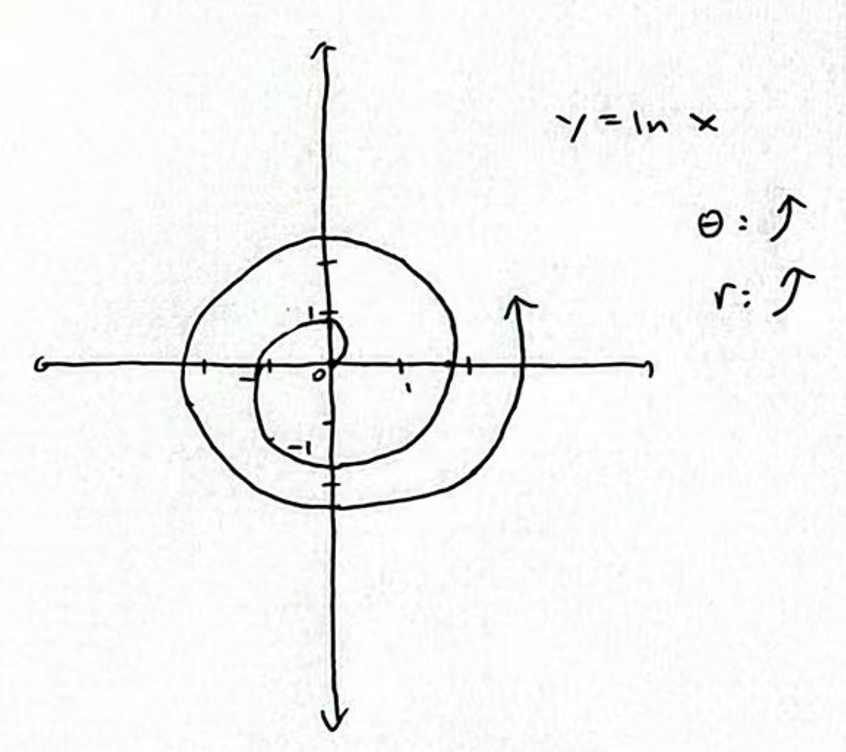
\includegraphics[width=0.5\linewidth]{屏幕截图 2026-02-18 080546.png}
    \caption{2.c}
    \label{fig:placeholder}
\end{figure}

\section{Question 3}
\subsection{(a)} \, Sketch the following curves using a table of values:

\vspace{-1.5em}
\begin{flalign*}
    & \textbf{i. } r=2\cos \theta &
\end{flalign*}

\begin{figure}[H]
    \centering
    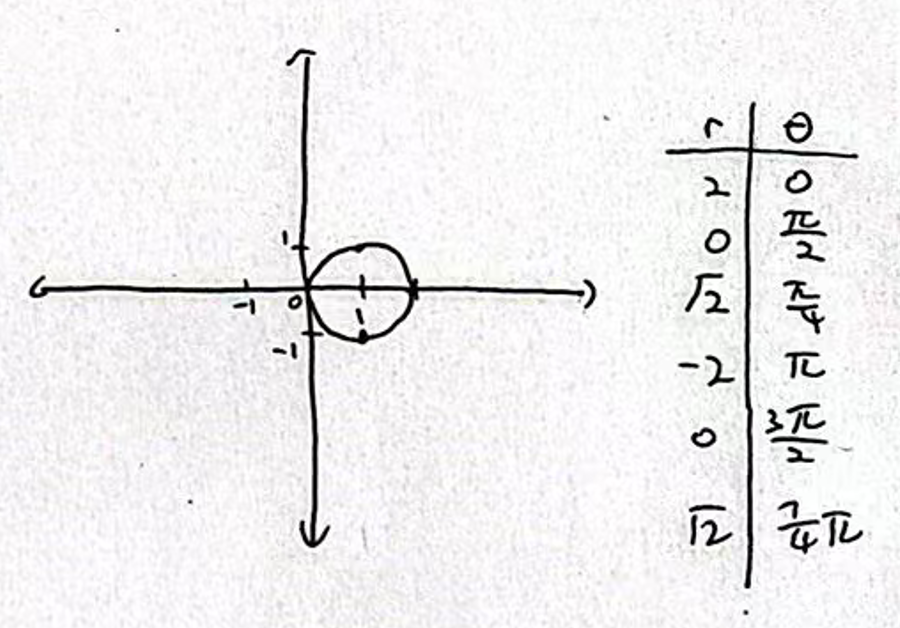
\includegraphics[width=0.5\linewidth]{屏幕截图 2026-02-18 080818.png}
    \caption{3.i.}
    \label{fig:placeholder}
\end{figure}

\theorem{Circle}{
\begin{itemize}
    \item $r = a \sin \theta$ or $r = a \cos \theta$
\end{itemize}
}

\vspace{-1.5em}
\begin{flalign*}
    & \textbf{ii. } r=1+ \sin \theta &
\end{flalign*}

\begin{figure}[H]
    \centering
    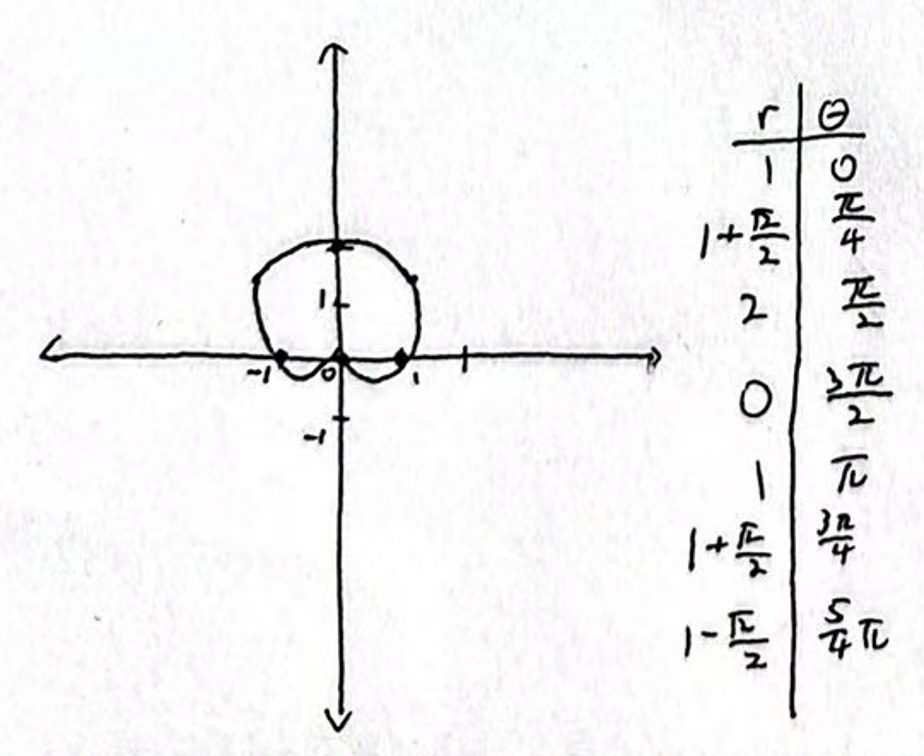
\includegraphics[width=0.5\linewidth]{屏幕截图 2026-02-18 081013.png}
    \caption{3.ii.}
    \label{fig:placeholder}
\end{figure}

\vspace{-1.5em}
\begin{flalign*}
    & \textbf{iii. } r=\cos 2\theta &
\end{flalign*}

\begin{figure}[H]
    \centering
    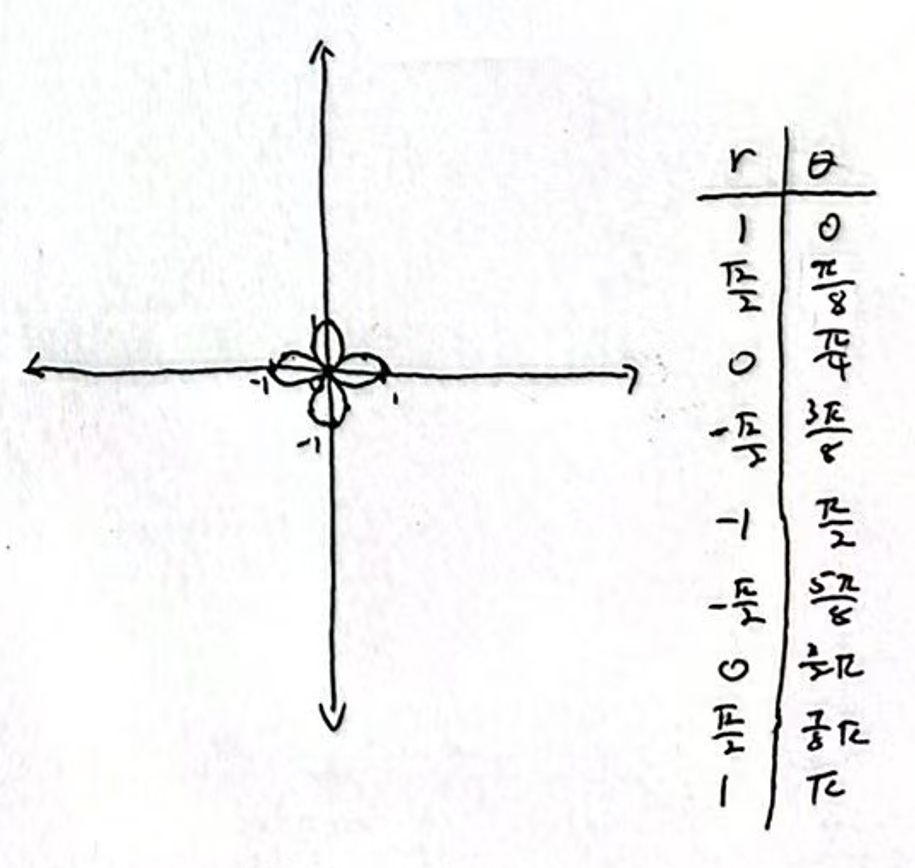
\includegraphics[width=0.5\linewidth]{屏幕截图 2026-02-18 081017.png}
    \caption{3.iii.}
    \label{fig:placeholder}
\end{figure}

\theorem{Rose Curve}{
\begin{itemize}
    \item $r = a \sin (n\theta)$ or $r = a \cos (n\theta)$
    \item $n$ even $\implies$ number of petals $= 2n$
    \item $n$ odd $\implies$ number of petals $= n$
\end{itemize}
}

\subsection{(b)} \, Find a Cartesian equation for each curve:
\begin{gather*}
    r=2\cos \theta \implies r^2 =2r \cos \theta \implies x^2+y^2=2x \implies \boxed{(x-1)^2+y^2=1}\\
    r=1+\sin \theta \implies (r^2 - r \sin \theta)^2 =  r^2 \implies \boxed{(x^2+y^2-y)^2=x^2+y^2}\\
    r=\cos 2\theta = \frac{r^2\cos^2 \theta -r^2\sin^2 \theta}{r^2} \implies \boxed{(x^2+y^2)^3=(x^2-y^2)^2}
\end{gather*}

\section{Question 4}
Consider symmetry rules of polar curves.

\theorem{Symmetry}
{\begin{itemize}
    \item Type 1: About polar axis (think x-axis) $\implies$ Replace $\theta$ by $(-\theta)$
    \item Type 2: About $\theta = \frac{\pi}{2}$ (think y-axis) $\implies$ Replace $\theta$ by $\pi-\theta$
    \item Type 3: Pole (think origin) $\implies$ Replace $(r, \theta)$ by either $(-r,\theta)$ or $(r, \theta+\pi)$
\end{itemize}}

\vspace{1em}
\section{Question 5}
Go back to problem $\#3$. Can the rule(s) discovered in problem $\#4$ speed up the sketching process in each case (i)-(iii)? If so, how? \\

If any of the above symmetry requirements regarding $\theta$ and $r$ are sustained, then the graph is guaranteed to be symmetric regarding the corresponding axis or points of symmetry. Thus, we may skip identical/symmetrical parts of the graph to increase efficiency. 

\vspace{1em}

\section{Question 6}
Sketch a graph of the following curves:

\vspace{-1.5em}
\begin{flalign*}
    & \textbf{(a) } r=2\cos 4 \theta &
\end{flalign*}

\begin{figure}[H]
    \centering
    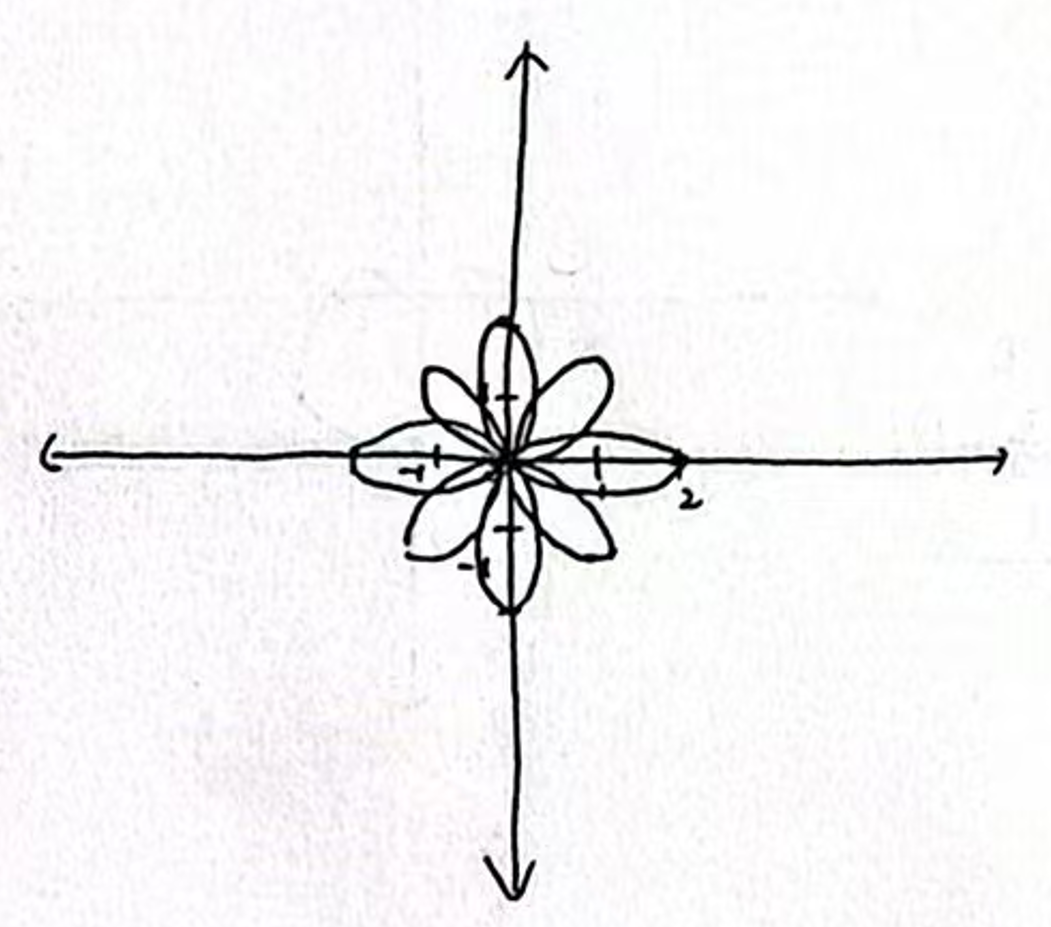
\includegraphics[width=0.5\linewidth]{屏幕截图 2026-02-18 114401.png}
    \caption{6.a}
    \label{fig:placeholder}
\end{figure}

\vspace{-1.5em}
\begin{flalign*}
    & \textbf{(c) } r=2 + \sin 3 \theta &
\end{flalign*}

\begin{figure}[H]
    \centering
    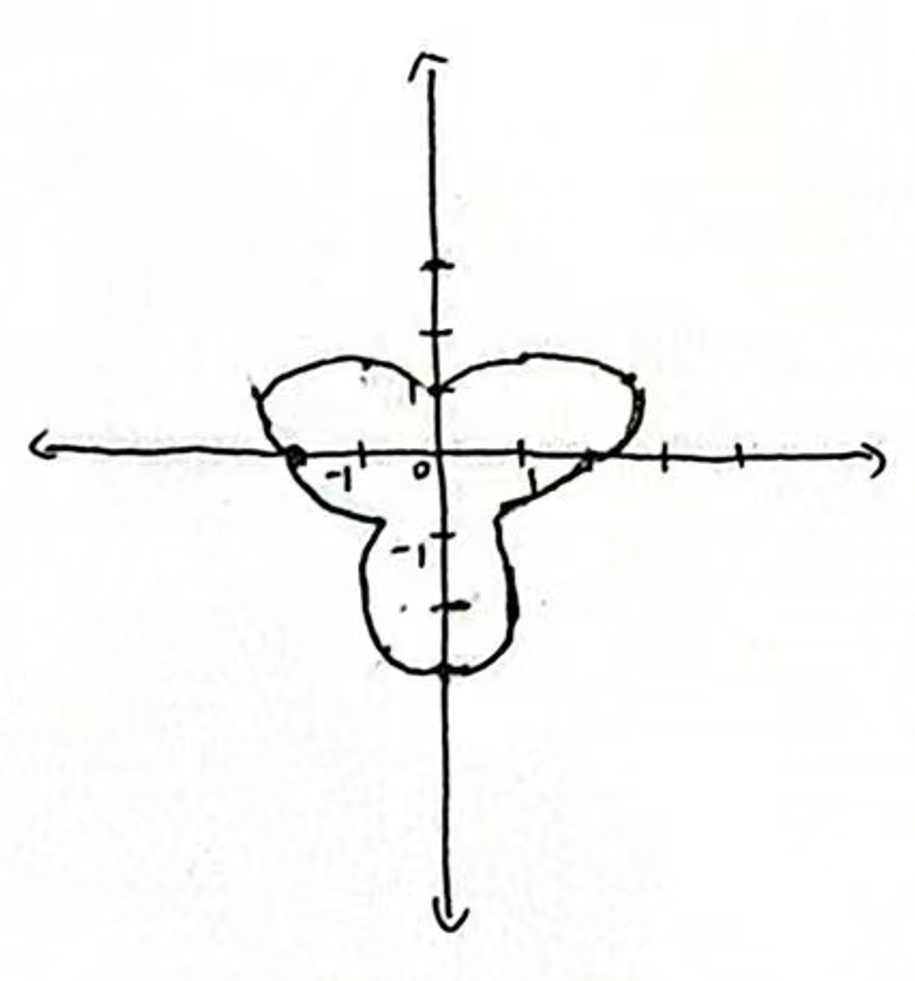
\includegraphics[width=0.5\linewidth]{屏幕截图 2026-02-18 114405.png}
    \caption{6.c}
    \label{fig:placeholder}
\end{figure}

\vspace{-1.5em}
\begin{flalign*}
    & \textbf{(d) } r=1 + 2\cos 2\theta &
\end{flalign*}

\begin{figure}[H]
    \centering
    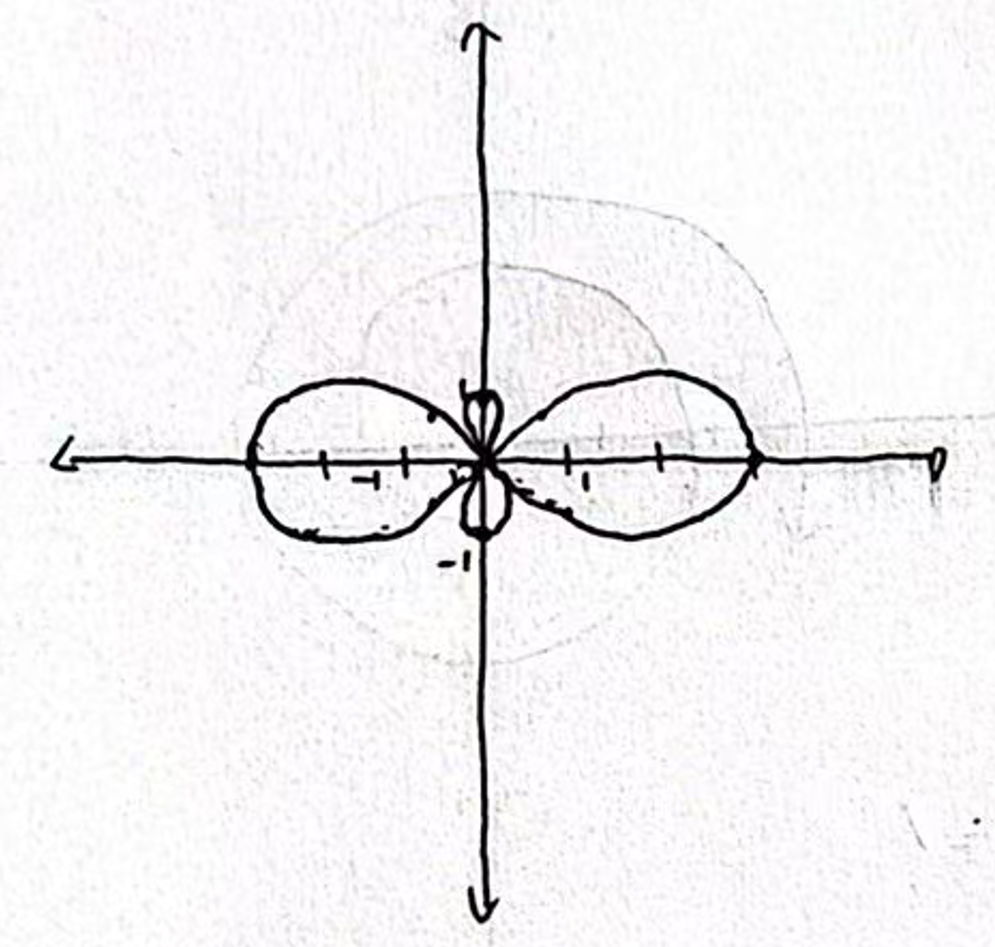
\includegraphics[width=0.5\linewidth]{屏幕截图 2026-02-18 114409.png}
    \caption{6.d}
    \label{fig:placeholder}
\end{figure}

\theorem{Lemniscate}{
\begin{itemize}
    \item $r^2 = a \sin (2\theta)$ or $r^2 = a \cos (2\theta)$
\end{itemize}
}

\section{Question 7}
The figure below shows the graph of $r$ as a function of $\theta$ in Cartesian coordinates. Use it to sketch the corresponding polar curve.
\begin{figure}[H]
    \centering
    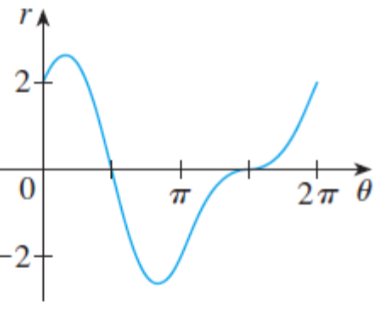
\includegraphics[width=0.25\linewidth]{屏幕截图 2026-02-18 115641.png}
    \caption{Question 7}
    \label{fig:placeholder}
\end{figure}

\begin{figure}
    \centering
    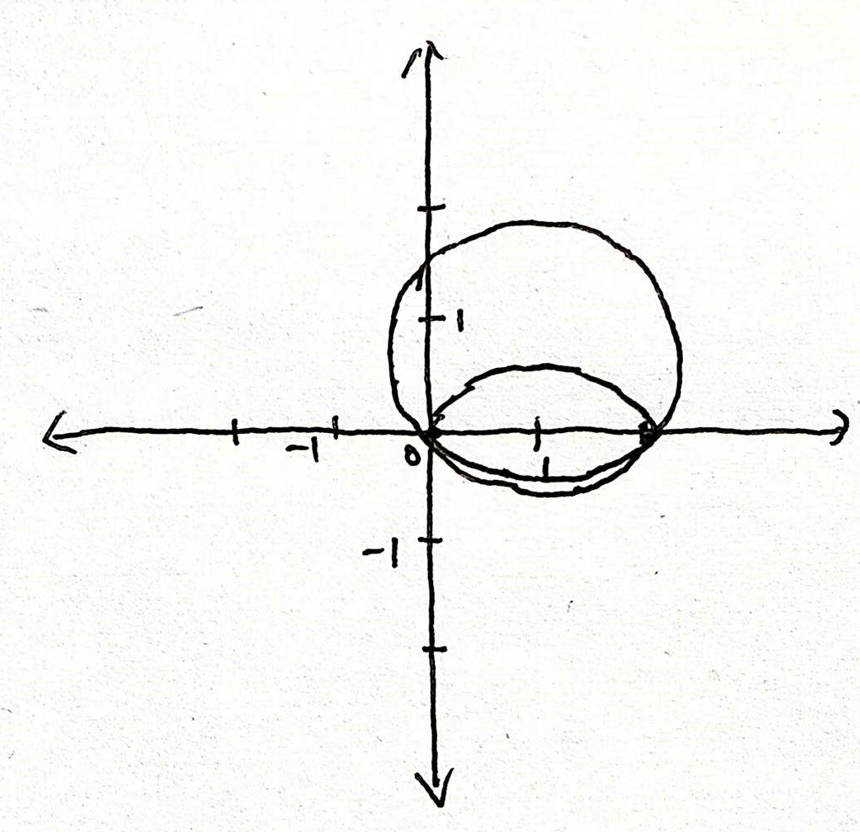
\includegraphics[width=0.5\linewidth]{屏幕截图 2026-02-20 080837.png}
    \caption{Solution 7}
    \label{fig:placeholder}
\end{figure}

\section{Question 8}
Show that the polar curve $r = 4 + 2 \sec \theta$ (called a conchoid) has the line $x = 2$ as a vertical asymptote
by showing that $\lim\limits_{r \to \pm \infty} x=2$.
Use this fact to help sketch the conchoid.
\begin{gather*}
    r = 4 + 2 \sec \theta \implies r\cos x=4 \cos \theta +2\implies x=4 \cos \theta +2\\
    r \to \pm \infty \implies \sec \theta \to \pm \infty \implies \cos \theta \to 0^{\pm}\\
    x=4\cos \theta +2=2
\end{gather*}

\begin{figure}[H]
    \centering
    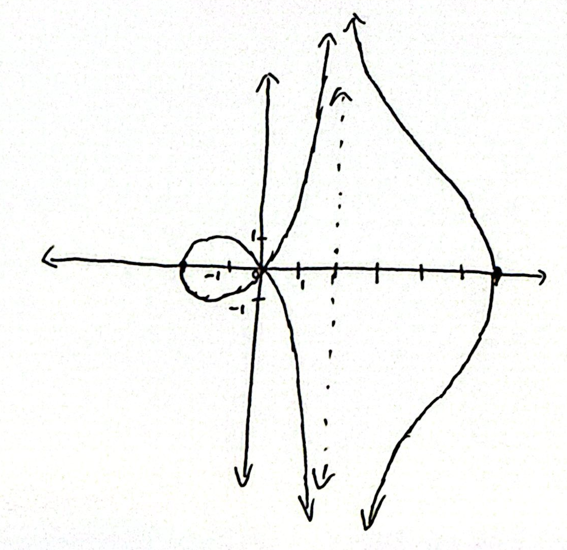
\includegraphics[width=0.5\linewidth]{Screenshot 2026-02-18 110101.png}
    \caption{Conchoid}
    \label{fig:placeholder}
\end{figure}

\section{Question 9}
Use a graphing tool to graph the polar curves:
\begin{flalign*}
    & \textbf{(a) } r=1+2\sin (\frac{\theta}{2}) \textbf{  (Nephroid of Freeth)} &
\end{flalign*} 

\begin{figure}[H]
    \centering
    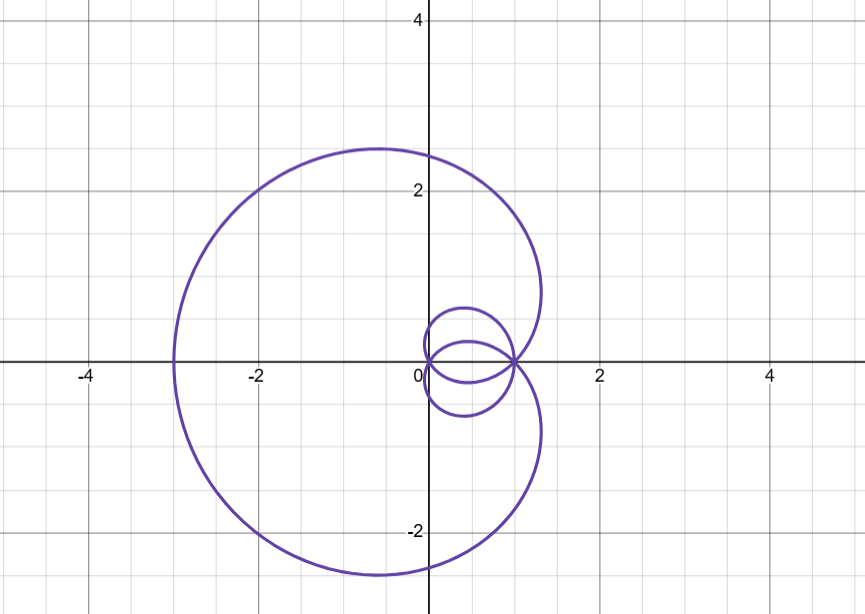
\includegraphics[width=0.5\linewidth]{Screenshot 2026-02-17 140651.png}
    \caption{Nephroid of Freeth}
    \label{fig:placeholder}
\end{figure}

\vspace{-1em}
\begin{flalign*}
    & \textbf{(b) } r=\sqrt{1-0.8\sin^2 \theta} \textbf{  (Hippopede)} &
\end{flalign*}

\begin{figure}[H]
    \centering
    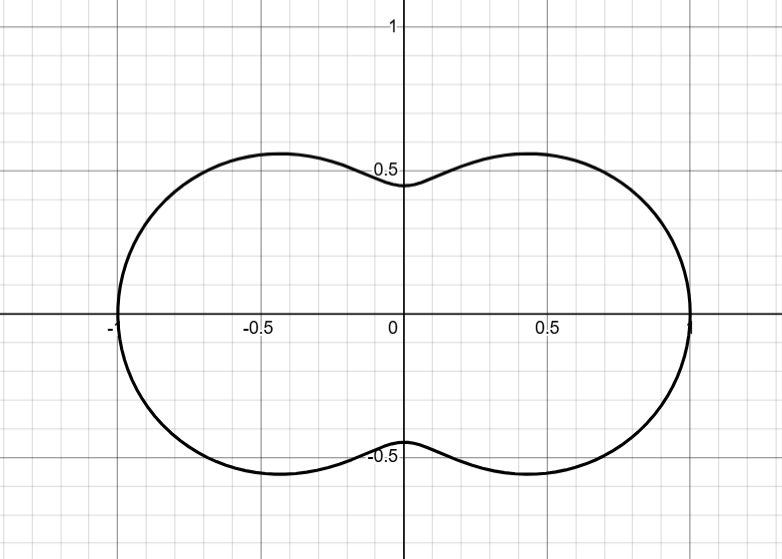
\includegraphics[width=0.5\linewidth]{Screenshot 2026-02-17 141038.png}
    \caption{Hippopede}
    \label{fig:placeholder}
\end{figure}

\vspace{-1em}
\begin{flalign*}
    & \textbf{(c) } r=e^{\sin \theta} -2\cos (4\theta) \textbf{  (Butterfly Curve)} &
\end{flalign*} 

\begin{figure}[H]
    \centering
    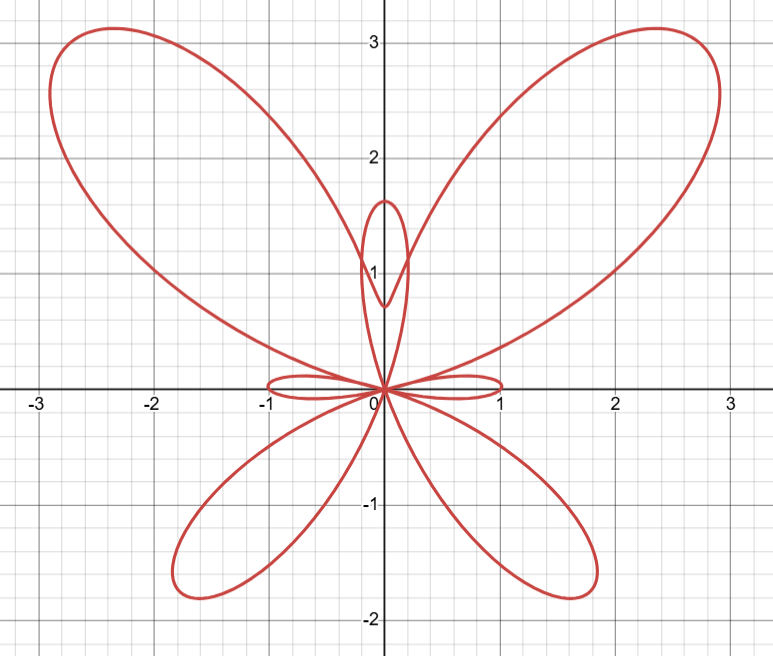
\includegraphics[width=0.5\linewidth]{Screenshot 2026-02-17 141151.png}
    \caption{Butterfly Curve}
    \label{fig:placeholder}
\end{figure}

\section{Question 10}
The astronomer Giovanni Cassini (1625-1712) studied the family of curves with polar equations $r^4 - 2c^2r^2 \cos 2\theta + c^4 - a^4 = 0$ where $a$ and $c$ are positive real numbers. These curves are called the ovals of Cassini even though they are oval-shaped only for certain values of $a$ and $c$. Cassini thought that these curves might represent planetary orbits better than Kepler’s ellipses. Investigate the variety of shapes that these curves may have. In particular, how are $a$ and $c$ related to each other when the curve splits into two parts?
\begin{gather*}
    r^4 - 2c^2r^2 \cos 2\theta + c^4 - a^4 =0\\
    (x^2+y^2)^2-2c^2(x^2-y^2)=a^4-c^4\\
    (x^2+y^2)^2+2c^2(x^2+y^2)-4c^2x^2=a^4-c^4\\
    (x^2+y^2+c^2)^2-4c^2x^2=a^4-c^4+c^4\\
    (x^2+y^2+c^2-2cx)(x^2+y^2+c^2+2cx)=a^4\\
    ((x-c)^2+y^2)((x+c)^2+y^2)=a^4
\end{gather*}

The product of the distances to the two foci 
$(c,0)$ and $(-c,0)$ is a constant $a^2$.

\theorem{Oval of Cassini}{
\begin{itemize}
    \item $\frac{a}{c}>1$: A single loop in oval shape or curved downwards towards the midpoint. 
    \item $\frac{a}{c}=1$: Lemniscate.
    \item $\frac{a}{c}<1$: Two separate loops each surrounding one of the two foci.
\end{itemize}
}

\end{document}

